\documentclass[letterpaper,10pt]{book}
% Change to 10 pt
\usepackage{pdfpages}
\usepackage{morewrites}			% to counteract the no write space problem
\setcounter{tocdepth}{6}

\usepackage[framemethod=TikZ]{mdframed}

\usepackage{fancyhdr}

\usepackage{paralist}
\usepackage{amsmath}
\usepackage{amsfonts}
\usepackage{amssymb}
\usepackage{graphicx}

\usepackage{datetime}
%\usepackage{ulem}

%\usepackage[nottoc]{toobibind}

\usepackage[inline]{enumitem}

% Outer margin at 2.50 is exacty correct to fit the ``corruption alert'' tables
\usepackage[inner=1.0in, outer=2.50in, top=2.54cm,bottom=2.54cm, marginparwidth=2.25in]{geometry}

\usepackage{marginnote}
\usepackage{longtable}
\usepackage{booktabs}
\usepackage{xcolor}

\usepackage{soul}

%%%%%%%%%%%%
\definecolor{ForestGreen}{rgb}{0.00,0.29,0.098}
%%%%%%%%%%%%

\usepackage{marginnote}

\usepackage{imakeidx} 
\usepackage[
	backref=true,
	style=numeric,
%	citestyle=numeric,
	backend=bibtex
	]{biblatex}
\usepackage[driverfallback=hypertex,colorlinks=True]{hyperref}
\usepackage{cleveref}

\makeindex[name=scripture,columnsep=20pt, columnseprule=True,columns=3, title=Scripture References]
\makeindex[name=speaker,columnsep=20pt, columnseprule=True,,columns=2, title=Sermon Creator]
\makeindex[name=series,columnsep=20pt, columnseprule=True,,columns=2, title=Sermon Series]
\makeindex[name=date,columnsep=20pt, columnseprule=True,columns=2, title=Sermon Date]
\makeindex[name=event,columnsep=20pt, columnseprule=True,columns=2, title=Event]
\makeindex[name=topic,columnsep=20pt, columnseprule=True,columns=2, title=Topic]
\makeindex[name=AWIP,columnsep=20pt, columnseprule=True,columns=3, title=All Words in Passage]
\makeindex[name=NWIV,columnsep=20pt, columnseprule=True,columns=3, title=Number of Words in Verse]
\makeindex[name=PNIP,columnsep=20pt, columnseprule=True,columns=3, title=Proper Names in Passage]
\makeindex[name=PEIP,columnsep=20pt, columnseprule=True,columns=2, title=Prophetic Events in Passage]
\makeindex[name=TWPAQ,columnsep=20pt, columnseprule=True,columns=1, title=13-Word Phrases and Quotes]
\makeindex[name=PFTTIS,columnsep=20pt, columnseprule=False,columns=3, title=Phrases found 13 times in scripture]
\makeindex[name=WFTTIS,columnsep=20pt, columnseprule=False,columns=3, title=Words found 13 times in scripture]
\makeindex[name=WFITV,columnsep=20pt, columnseprule=False,columns=3, title=Words found in exactly 13 verses]
\makeindex[name=EVENTS,columnsep=20pt, columnseprule=False,columns=2, title=Sermon Log by Place]
\makeindex[name=QUESTIONS,columnsep=20pt, columnseprule=False,columns=2, title=Bible Questions]
\makeindex[name=DOCTRINES,columnsep=20pt, columnseprule=False,columns=2, title=Doctrines]
\makeindex[name=SONGS,columnsep=20pt, columnseprule=False,columns=1, title=Songs]
\makeindex[name=LOCATION,columnsep=20pt, columnseprule=False,columns= 2, title=Location]
\makeindex[name=FACEBOOK,columnsep=20pt, columnseprule=False,columns=2, title=Facebook]
\makeindex[name=DEVOTIONAL,columnsep=20pt, columnseprule=False,columns=2, title=Devotional Items]
%%%%%%%%%%%%%%%%% EXTRA COLORS
\definecolor{champagne}{rgb}{0.97,0.91,0.81}
\definecolor{bone}{rgb}{0.89,0.85,0.79}
\pagestyle{fancy}
\fancyhf{}
\fancyhead[LE,RO]{\today}
\fancyhead[RE,LO]{Daily Bible Reading}
\fancyhead[CE,CO]{-page \thepage  - }

\fancyfoot[CO,CE]{\leftmark}
%\fancyfoot[LE,RO]{CSCE 692, HW1}

\title{DBR\\
Daily \\ Reads}
\author{Keith Anthony \\
\today }
%+/ffffff +   \pagenumbering{gobble}
\bibliography{Bibliographies/All20220122}

\setlength{\fboxsep}{1.0pt}

\usepackage[utf8]{inputenc}
\usepackage{tikz}

\begin{document}
%%%%%%%%%%%% Tile Page

\begin{titlepage}

\begin{flushright}
\rightskip=-2.5cm
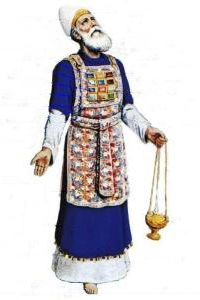
\includegraphics[width=50mm,scale=1.5]{Extras/Melchisedec.jpg}
\vspace{0.4in}  % Create a title for the document and write it in bold font
\LARGE{\textbf{\date}} % Again, do a line break
\linebreak 
% Create a subtitle \large{with Outlines, Statistics, Cross References, and Notes}
\vspace{0.5in}
\begin{flushleft}
\LARGE{Day \#78: Saturday, 19  March 2022 PLAIN  \\}\vspace{0.25in}
\LARGE{Judges 16-18 Psalm 78 Proverb 19}
\end{flushleft}
\vspace{0.6in}
\bigskip

\normalsize{Xenia, Oh.\\}
\normalsize{created: \today}
\vspace{1.3in}

\end{flushright}
\end{titlepage}

\newpage 
\tableofcontents\hypertarget{TOC}{}
\listoffigures
\listoftables

\hyphenation{A-bim-e-lech bre-thren E-phra-im  Gib-e-o-nites Jer-u-sa-lem through-out Phil-i-stines The-o-phil-us Am-a-le-kites ven-geance Mesh-el-e-mi-ah onan-ism Phar-a-oh thoughts grev-ous-ness Hach-a-liah adul-ter-er Shad-rach}

%%%%%%%%%%%%%%%%% EXTRA COLORS
%%%%%%%%%%%%%%%%% EXTRA COLORS
%%%%%%%%%%%%%%%%% EXTRA COLORS
\definecolor{champagne}{rgb}{0.97,0.91,0.81}
\definecolor{bone}{rgb}{0.89,0.85,0.79}

\definecolor{ForestGreen}{rgb}{0.00,0.29,0.098}
\definecolor{GIVING}{cmyk}{1,0.0,0.72,.1}

\definecolor{MLPE}{cmyk}{1,1,0,.45}
\definecolor{SOCCER}{cmyk}{.77, 0, .42, .49}
\definecolor{PAYBILL}{cmyk}{0,0.83,0.76,0.07}
\definecolor{SERMON}{cmyk}{.14,.9,0,.30} % aka seance \href{http://www.flatuicolorpicker.com/purple-cmyk-color-model/}{seance}
\definecolor{BIBLE}{cmyk}{0,.17,.74,.17}
\definecolor{WORKBLUE}{cmyk}{1, .5, 0, .6}
\definecolor{myOrange}{cmyk}{0, .4, .98, .03}
\definecolor{myTan}{cmyk}{0.0,.07,.17,.10}
\definecolor{myRed}{cmyk}{0,1,1,0}
\definecolor{myWhite}{cmyk}{0,0,0,0}
\definecolor{BLUESoD}{cmyk}{.97,.84,0,.04}
\definecolor{WHITE}{cmyk}{0,0,0,0}
\definecolor{OLDGOLD}{cmyk}{0.05,0.3,1.00,0}
\definecolor{CASTLETON}{cmyk}{1,0,0.31,0.66}
\definecolor{cadmiumgreen}{rgb}{0.0, 0.42, 0.24}
\definecolor{jungle}{rgb}{0.203,0.4882,0.1718}
\definecolor{MYGOLD}{rgb}{1,.84,0}

\definecolor{MYLIGHTGRAY}{rgb}{.85,.85,.85}

\definecolor{codegreen}{rgb}{0,0.6,0}
\definecolor{codegray}{rgb}{0.5,0.5,0.5}
\definecolor{codepurple}{rgb}{0.58,0,0.82}
\definecolor{backcolour}{rgb}{0.95,0.95,0.92}


\mdfdefinestyle{MyFrame}{%
    linecolor=blue,
    outerlinewidth=2pt,
    roundcorner=5pt,
    innertopmargin=\baselineskip,
    innerbottommargin=\baselineskip,
    innerrightmargin=10pt,
    innerleftmargin=10pt,
    backgroundcolor=gray!25!white}


\mdfdefinestyle{MyFrame2}{%
    linecolor=black,
    outerlinewidth=2pt,
    roundcorner=5pt,
    innertopmargin=\baselineskip,
    innerbottommargin=\baselineskip,
    innerrightmargin=10pt,
    innerleftmargin=10pt,
    backgroundcolor=yellow!25!white}


%%%%%
%% for PFTTIS list
%%%%%

%%% And Joseph said unto
\index[PFTTIS]{And Joseph said unto!Genesis!Gen 40:008}
\index[PFTTIS]{And Joseph said unto!Genesis!Gen 40:012}
\index[PFTTIS]{And Joseph said unto!Genesis!Gen 41:025}
\index[PFTTIS]{And Joseph said unto!Genesis!Gen 42:014}
\index[PFTTIS]{And Joseph said unto!Genesis!Gen 42:018}
\index[PFTTIS]{And Joseph said unto!Genesis!Gen 44:015}
\index[PFTTIS]{And Joseph said unto!Genesis!Gen 45:003}
\index[PFTTIS]{And Joseph said unto!Genesis!Gen 45:004}
\index[PFTTIS]{And Joseph said unto!Genesis!Gen 46:031}
\index[PFTTIS]{And Joseph said unto!Genesis!Gen 48:009}
\index[PFTTIS]{And Joseph said unto!Genesis!Gen 48:018}
\index[PFTTIS]{And Joseph said unto!Genesis!Gen 50:019}
\index[PFTTIS]{And Joseph said unto!Genesis!Gen 50:024}


%%% a shadow
\index[PFTTIS]{a shadow!1Chronicles!1Chr 029:15}
\index[PFTTIS]{a shadow!Job!Job 008:09}
\index[PFTTIS]{a shadow!Job!Job 014:02}
\index[PFTTIS]{a shadow!Job!Job 017:07}
\index[PFTTIS]{a shadow!Psalm!Psa 102:011}
\index[PFTTIS]{a shadow!Psalm!Psa 144:004}
\index[PFTTIS]{a shadow!Ecclesiastes!Eccl 006:012}
\index[PFTTIS]{a shadow!Ecclesiastes!Eccl 008:013}
\index[PFTTIS]{a shadow!Isaiah!Isa 04:006}
\index[PFTTIS]{a shadow!Isaiah!Isa 25:004}
\index[PFTTIS]{a shadow!Jonah!Jnh 04:06}
\index[PFTTIS]{a shadow!Colossians!Col 02:017}
\index[PFTTIS]{a shadow!Hebews!Heb 10:001}

%%% blessed is the man
\index[PFTTIS]{blessed is the man!Psalm!Psa 001:001}
\index[PFTTIS]{blessed is the man!Psalm!Psa 032:002}
\index[PFTTIS]{blessed is the man!Psalm!Psa 034:008}
\index[PFTTIS]{blessed is the man!Psalm!Psa 065:004}
\index[PFTTIS]{blessed is the man!Psalm!Psa 084:005}
\index[PFTTIS]{blessed is the man!Psalm!Psa 084:012}
\index[PFTTIS]{blessed is the man!Psalm!Psa 094:012}
\index[PFTTIS]{blessed is the man!Psalm!Psa 112:001}
\index[PFTTIS]{blessed is the man!Proverbs!Pro 008:034}
\index[PFTTIS]{blessed is the man!Isaiah!Isa 056:002}
\index[PFTTIS]{blessed is the man!Jeremiah!Jer 017:007}
\index[PFTTIS]{blessed is the man!Romans!Rom 004:008}
\index[PFTTIS]{blessed is the man!James!Jam 001:012}


%%% carry them
\index[PFTTIS]{carry them!Leviticus!Lev 14:045}
\index[PFTTIS]{carry them!Numbers!Num 11:012}
\index[PFTTIS]{carry them!Joshua!Jsh 04:003}
\index[PFTTIS]{carry them!1Samuel!1Sam 20:040}
\index[PFTTIS]{carry them!1Kings!1Kng 08:046}
\index[PFTTIS]{carry them!2Chronicles!2Chr 06:036}
\index[PFTTIS]{carry them!Ezra!Ezra 05:015}
\index[PFTTIS]{carry them!Isaiah!Isa 40:011}
\index[PFTTIS]{carry them!Isaiah!Isa 41:016}
\index[PFTTIS]{carry them!Isaiah!Isa 57:013}
\index[PFTTIS]{carry them!Jeremiah!Jer 20:004}
\index[PFTTIS]{carry them!Jeremiah!Jer 20:005}
\index[PFTTIS]{carry them!Jeremiah!Jer 43:012}


\index[PFTTIS]{good tidings!2Samuel!2Sam 18:027}
\index[PFTTIS]{good tidings!1Kings!1Ki 01:042}
\index[PFTTIS]{good tidings!2Kings!2Ki 07:009 (2x)}
\index[PFTTIS]{good tidings!Isaiah!Isa 40:009 (2x)}
\index[PFTTIS]{good tidings!Isaiah!Isa 41:007}
\index[PFTTIS]{good tidings!Isaiah!Isa 52:007}
\index[PFTTIS]{good tidings!Isaiah!Isa 61:001}
\index[PFTTIS]{good tidings!Nahum!Nah 01:005}
\index[PFTTIS]{good tidings!Luke!Lk 02:010}
\index[PFTTIS]{good tidings!1Thessalonians!1Thess 03:006}


%%% dead body
\index[PFTTIS]{dead body!Leviticus!Lev 21:011}
\index[PFTTIS]{dead body!Numbers!Num 06:006}
\index[PFTTIS]{dead body!Numbers!Num 09:006}
\index[PFTTIS]{dead body!Numbers!Num 09:007}
\index[PFTTIS]{dead body!Numbers!Num 09:010}
\index[PFTTIS]{dead body!Numbers!Num 09:011}
\index[PFTTIS]{dead body!Numbers!Num 09:013}
\index[PFTTIS]{dead body!Numbers!Num 09:016}
\index[PFTTIS]{dead body!2Kings!2Ki 08:005}
\index[PFTTIS]{dead body!Isaiah!Isa 26:019}
\index[PFTTIS]{dead body!Jeremiah!Jer 26:023}
\index[PFTTIS]{dead body!Jeremiah!Jer 36:030}
\index[PFTTIS]{dead body!Haggai!Hag 02:013}

%%% great sea
\index[PFTTIS]{great sea!Numbers!Num 34:006}
\index[PFTTIS]{great sea!Numbers!Num 34:007}
\index[PFTTIS]{great sea!Joshua!Jos 01:004}
\index[PFTTIS]{great sea!Joshua!Jos 09:001}
\index[PFTTIS]{great sea!Joshua!Jos 15:012}
\index[PFTTIS]{great sea!Joshua!Jos 15:047}
\index[PFTTIS]{great sea!Joshua!Jos 23:004}
\index[PFTTIS]{great sea!Ezekiel!Eze 47:010}
\index[PFTTIS]{great sea!Ezekiel!Eze 47:015}
\index[PFTTIS]{great sea!Ezekiel!Eze 47:019}
\index[PFTTIS]{great sea!Ezekiel!Eze 47:020}
\index[PFTTIS]{great sea!Ezekiel!Eze 48:028}
\index[PFTTIS]{great sea!Daniel!Dan 07:002}


%%% have forsaken me
\index[PFTTIS]{have forsaken me!Judges!Jdg 10:013}
\index[PFTTIS]{have forsaken me!1Samuel!1Sam 08:008}
\index[PFTTIS]{have forsaken me!1Kings!1Ki 11:033}
\index[PFTTIS]{have forsaken me!2Kings!2Ki 22:017}
\index[PFTTIS]{have forsaken me!2Chronicles!2Chr 12:005}
\index[PFTTIS]{have forsaken me!2Chronicles!2Chr 34:025}
\index[PFTTIS]{have forsaken me!Jeremiah!Jer 01:016}
\index[PFTTIS]{have forsaken me!Jeremiah!Jer 02:013}
\index[PFTTIS]{have forsaken me!Jeremiah!Jer 05:007}
\index[PFTTIS]{have forsaken me!Jeremiah!Jer 05:019}
\index[PFTTIS]{have forsaken me!Jeremiah!Jer 16:011 (2x)}
\index[PFTTIS]{have forsaken me!Jeremiah!Jer 19:004}

%%% no king
\index[PFTTIS]{no king!Judges!Jdg 17:06}
\index[PFTTIS]{no king!Judges!Jdg 18:01}
\index[PFTTIS]{no king!Judges!Jdg 19:01}
\index[PFTTIS]{no king!Judges!Jdg 21:25}
\index[PFTTIS]{no king!1Kings!1Ki 22:47}
\index[PFTTIS]{no king!2Kings!2Ki 23:25}
\index[PFTTIS]{no king!Nehemiah!Neh 13:26}
\index[PFTTIS]{no king!Psalms!Psa 033:016}
\index[PFTTIS]{no king!Proverbs!Pro 30:27}
\index[PFTTIS]{no king!Daniel!Dan 02:10}
\index[PFTTIS]{no king!Hosea!Hos 10:03}
\index[PFTTIS]{no king!Micah!Mic 04:09}
\index[PFTTIS]{no king!John!Jhn 19:15}


%%% rebellious house
\index[PFTTIS]{rebellious house!Exodus!Exo 02:005}
\index[PFTTIS]{rebellious house!Exodus!Exo 02:006}
\index[PFTTIS]{rebellious house!Exodus!Exo 02:008}
\index[PFTTIS]{rebellious house!Exodus!Exo 03:009}
\index[PFTTIS]{rebellious house!Exodus!Exo 03:026}
\index[PFTTIS]{rebellious house!Exodus!Exo 03:027}
\index[PFTTIS]{rebellious house!Exodus!Exo 12:002 (2x)}
\index[PFTTIS]{rebellious house!Exodus!Exo 12:003}
\index[PFTTIS]{rebellious house!Exodus!Exo 12:009}
\index[PFTTIS]{rebellious house!Exodus!Exo 12:025}
\index[PFTTIS]{rebellious house!Exodus!Exo 17:012}
\index[PFTTIS]{rebellious house!Exodus!Exo 24:003}

%%% seek him
\index[PFTTIS]{seek him!Deuteronomy!Deu 04:029}\index[PFTTIS]{seek him!1Samuel!1Sam 23:025}
\index[PFTTIS]{seek him!1Chronicles!1Chr 28:009}
\index[PFTTIS]{seek him!2Chronicles!1Chr 15:002}
\index[PFTTIS]{seek him!Ezra!Ezr 08:022}
\index[PFTTIS]{seek him!Psalms!Psa 022:026}
\index[PFTTIS]{seek him!Psalms!Psa 024:006}
\index[PFTTIS]{seek him!Psalms!Psa 119:002}
\index[PFTTIS]{seek him!SoS!SoS 03:002}
\index[PFTTIS]{seek him!SoS!SoS 06:001}
\index[PFTTIS]{seek him!Hosea!Hos 07:010}
\index[PFTTIS]{seek him!Amos!Amo 05:008}
\index[PFTTIS]{seek him!Hebrews!Heb 11:0063}


%%% seek ye
\index[PFTTIS]{seek ye!Isaiah!Isa 34:016}
\index[PFTTIS]{seek ye!Isaiah!Isa 45:019}
\index[PFTTIS]{seek ye!Isaiah!Isa 55:006}
\index[PFTTIS]{seek ye!Amos!Amos 5:004}
\index[PFTTIS]{seek ye!John!John 1:38}
\index[PFTTIS]{seek ye!John!John 18:4}
\index[PFTTIS]{seek ye!John!John 18:7}
\index[PFTTIS]{seek ye!Matthew!Matt 6:33}
\index[PFTTIS]{seek ye!Numbers!Num 16:10}
\index[PFTTIS]{seek ye!Luke!Luke 12:31}
\index[PFTTIS]{seek ye!Luke!Luke 24:5}
\index[PFTTIS]{seek ye!Psalm!Psa 27:8}
\index[PFTTIS]{seek ye!Zephaniah!Zeph 2:3}

%%% the uncircumcised
\index[PFTTIS]{the uncircumcised!Genesis!Gen 17:014}
\index[PFTTIS]{the uncircumcised!Judges!Jdg 14:003}
\index[PFTTIS]{the uncircumcised!Judges!Jdg 15:018}
\index[PFTTIS]{the uncircumcised!2Samuel!2Sam 01:020}
\index[PFTTIS]{the uncircumcised!Isaiah!Isa 02:001}
\index[PFTTIS]{the uncircumcised!Jeremiah!Jer 09:025}
\index[PFTTIS]{the uncircumcised!Ezekiel!Eze 28:010}
\index[PFTTIS]{the uncircumcised!Ezekiel!Eze 31:018}
\index[PFTTIS]{the uncircumcised!Ezekiel!Eze 32:019}
\index[PFTTIS]{the uncircumcised!Ezekiel!Eze 32:027}
\index[PFTTIS]{the uncircumcised!Ezekiel!Eze 32:028}
\index[PFTTIS]{the uncircumcised!Ezekiel!Eze 32:029}
\index[PFTTIS]{the uncircumcised!Ezekiel!Eze 32:032}

%%% worship him
\index[PFTTIS]{worship him!Psalms!Psa 97:007}
\index[PFTTIS]{worship him!Zephaniah!Zeph 02:011}
\index[PFTTIS]{worship him!Matthew!Matt 02:002}
\index[PFTTIS]{worship him!Matthew!Matt 02:008}
\index[PFTTIS]{worship him!John!John 04:023}
\index[PFTTIS]{worship him!John!John 04:024 (2x)} 
\index[PFTTIS]{worship him!Acts!Acts 17:023}
\index[PFTTIS]{worship him!Hebrews!Heb 01:006}
\index[PFTTIS]{worship him!Revelation!Rev 04:010}
\index[PFTTIS]{worship him!Revelation!Rev 13:008}
\index[PFTTIS]{worship him!Revelation!Rev 14:007}
\index[PFTTIS]{worship him!Revelation!Rev 19:010}


%%%%%
%% for PFTTIS list
%%%%%

%%% afflictions
\index[WFTTIS]{afflictions!Psalms!Psa 34:019}
\index[WFTTIS]{afflictions!Psalms!Psa 132:001}
\index[WFTTIS]{afflictions!Acts!Acts 07:010}
\index[WFTTIS]{afflictions!Acts!Acts 20:023}
\index[WFTTIS]{afflictions!2Corinthians!2Cor 06:004}
\index[WFTTIS]{afflictions!Colossians!Col 01:024}
\index[WFTTIS]{afflictions!1Thessalonians!1Thess 03:003}
\index[WFTTIS]{afflictions!2Timothy!2Tim 01:008}
\index[WFTTIS]{afflictions!2Timothy!2Tim 03:011}
\index[WFTTIS]{afflictions!2Timothy!2Tim 04:005}
\index[WFTTIS]{afflictions!Hebrews!Heb 10:032}
\index[WFTTIS]{afflictions!Hebrews!Heb 10:033}
\index[WFTTIS]{afflictions!1Peter!1Pet 05:009}

%%% acsend
\index[WFTTIS]{acsend!Joshua!Jos 06:05}
\index[WFTTIS]{acsend!Psalm!Psa 024:003}
\index[WFTTIS]{acsend!Psalm!Psa 135:007}
\index[WFTTIS]{acsend!Psalm!Psa 139:008}
\index[WFTTIS]{acsend!Isaiah!Isa 14:013}
\index[WFTTIS]{acsend!Isaiah!Isa 14:014}
\index[WFTTIS]{acsend!Jeremiah!Jer 10:013}
\index[WFTTIS]{acsend!Jeremiah!Jer 51:016}
\index[WFTTIS]{acsend!Ezekiel!Eze 38:009}
\index[WFTTIS]{acsend!John!John 06:062}
\index[WFTTIS]{acsend!John!John 20:017}
\index[WFTTIS]{acsend!Romans!Rom 10:006}
\index[WFTTIS]{acsend!Revelation!Rev 17:008}

%%% Assyrian
\index[WFTTIS]{Assyrian!Isaiah!Isa 10:005}
\index[WFTTIS]{Assyrian!Isaiah!Isa 10:024}
\index[WFTTIS]{Assyrian!Isaiah!Isa 14:025}
\index[WFTTIS]{Assyrian!Isaiah!Isa 19:023}
\index[WFTTIS]{Assyrian!Isaiah!Isa 23:013}
\index[WFTTIS]{Assyrian!Isaiah!Isa 30:031}
\index[WFTTIS]{Assyrian!Isaiah!Isa 31:008}
\index[WFTTIS]{Assyrian!Isaiah!Isa 52:004}
\index[WFTTIS]{Assyrian!Ezekiel!Eze 31:003}
\index[WFTTIS]{Assyrian!Hosea!Hos 05:013}
\index[WFTTIS]{Assyrian!Hosea!Hos 11:005}
\index[WFTTIS]{Assyrian!Micah!Hos 05:005}
\index[WFTTIS]{Assyrian!Micah!Hos 05:006}

%%% blot
\index[WFTTIS]{blot!Exodus!Exo 32:032}
\index[WFTTIS]{blot!Exodus!Exo 32:033}
\index[WFTTIS]{blot!Numbers!Num 05:026}
\index[WFTTIS]{blot!Deuteronomy!Deut 09:014}
\index[WFTTIS]{blot!Deuteronomy!Deut 25:019}
\index[WFTTIS]{blot!Deuteronomy!Deut 29:020}
\index[WFTTIS]{blot!2Kings!2Ki 14:027}
\index[WFTTIS]{blot!Job!Job 31:007}
\index[WFTTIS]{blot!Psalms!Psa 51:001}
\index[WFTTIS]{blot!Psalms!Psa 51:009}
\index[WFTTIS]{blot!Proverbs!Pro 09:007}
\index[WFTTIS]{blot!Jeremiah!Jer 18:023}
\index[WFTTIS]{blot!Revelation!Rev 03:005}


%%% chain
\index[WFTTIS]{chain!Genesis!Gen 41:042}
\index[WFTTIS]{chain!1Kings!1Ki 07:017}
\index[WFTTIS]{chain!Psalms!Psa 73:006}
\index[WFTTIS]{chain!SoS!Sos 04:009}
\index[WFTTIS]{chain!Lamentations!Lam 03:007}
\index[WFTTIS]{chain!Ezekiel!Eze 07:023}
\index[WFTTIS]{chain!Ezekiel!Eze 16:011}
\index[WFTTIS]{chain!Daniel!Dan 05:007}
\index[WFTTIS]{chain!Daniel!Dan 05:016}
\index[WFTTIS]{chain!Daniel!Dan 05:029}
\index[WFTTIS]{chain!Acts!Acts 28:020}
\index[WFTTIS]{chain!2Timothy!2Tim 01:016}
\index[WFTTIS]{chain!Revelation!Rev 20:001}


%%% controversy
\index[WFTTIS]{controversy!Deuteronomy!Deu 17:008}
\index[WFTTIS]{controversy!Deuteronomy!Deu 19:017}
\index[WFTTIS]{controversy!Deuteronomy!Deu 21:005}
\index[WFTTIS]{controversy!Deuteronomy!Deu 25:001}
\index[WFTTIS]{controversy!2Samuel!2Sam 15:002}
\index[WFTTIS]{controversy!Isaiah!Isa 34:008}
\index[WFTTIS]{controversy!Jeremiah!Jer 25:031}
\index[WFTTIS]{controversy!Ezekiel!Eze 44:024}
\index[WFTTIS]{controversy!Hosea!Hos 04:001}
\index[WFTTIS]{controversy!Hosea!Hos 12:002}
\index[WFTTIS]{controversy!Micah!Mic 06:002 (2x)}
\index[WFTTIS]{controversy!1Timothy!1Tim 03:016}


%%% Dagon/Dagon's
\index[WFTTIS]{Dagon!Judges!Jdg 16:023}
\index[WFTTIS]{Dagon!1Samuel!1Sam 05:002 (2x)}
\index[WFTTIS]{Dagon!1Samuel!1Sam 05:003 (2x)}
\index[WFTTIS]{Dagon!1Samuel!1Sam 05:004 (3x)}
\index[WFTTIS]{Dagon!1Samuel!1Sam 05:005 (3x)}
\index[WFTTIS]{Dagon!1Samuel!1Sam 05:007}
\index[WFTTIS]{Dagon!1Chronicles!1Chr 10:010}

%%% disobedient
\index[WFTTIS]{disobedient!1Kings!1Ki 13:026}
\index[WFTTIS]{disobedient!Nehemiah!Neh 09:026}
\index[WFTTIS]{disobedient!Luke!Luke 01:017}
\index[WFTTIS]{disobedient!Acts!Acts 26:019}
\index[WFTTIS]{disobedient!Romans!Rom 01:030}
\index[WFTTIS]{disobedient!Romans!Rom 10:021}
\index[WFTTIS]{disobedient!1Timothy!1Tim 01:009}
\index[WFTTIS]{disobedient!2Timothy!2Tim 03:002}
\index[WFTTIS]{disobedient!Titus!Titus 01:016}
\index[WFTTIS]{disobedient!Titus!Titus 03:003}
\index[WFTTIS]{disobedient!1Peter!1Pet 02:007}
\index[WFTTIS]{disobedient!1Peter!1Pet 02:008}
\index[WFTTIS]{disobedient!1Peter!1Pet 03:020}


%%% doubt
\index[WFTTIS]{doubt!Genesis!Gen 37:033}
\index[WFTTIS]{doubt!Deuteronomy!Deu 28:066}
\index[WFTTIS]{doubt!Job!Job 12:002}
\index[WFTTIS]{doubt!Matthew!Matt 14:031}
\index[WFTTIS]{doubt!Matthew!Matt 21:021}
\index[WFTTIS]{doubt!Mark!Mk 11:023}
\index[WFTTIS]{doubt!Luke!Lk 11:020}
\index[WFTTIS]{doubt!John!Jhn 10:024}
\index[WFTTIS]{doubt!Acts!Acts 02:012}
\index[WFTTIS]{doubt!Acts!Acts 28:004}
\index[WFTTIS]{doubt!1Corinthians!1Cor 09:010}
\index[WFTTIS]{doubt!Galatians!Gal 04:020}
\index[WFTTIS]{doubt!1John!1Jhn 02:019}


%%% dungeon
\index[WFTTIS]{dungeon!Genesis!Gen 40:015}
\index[WFTTIS]{dungeon!Genesis!Gen 41:014}
\index[WFTTIS]{dungeon!Exodus!Exo 12:029}
\index[WFTTIS]{dungeon!Jeremiah!Jer 37:016}
\index[WFTTIS]{dungeon!Jeremiah!Jer 38:006 (2x)}
\index[WFTTIS]{dungeon!Jeremiah!Jer 38:007}
\index[WFTTIS]{dungeon!Jeremiah!Jer 38:009}
\index[WFTTIS]{dungeon!Jeremiah!Jer 38:010}
\index[WFTTIS]{dungeon!Jeremiah!Jer 38:011}
\index[WFTTIS]{dungeon!Jeremiah!Jer 38:013}
\index[WFTTIS]{dungeon!Lamentations!Lam 03:053}
\index[WFTTIS]{dungeon!Lamentations!Lam 03:055}


%%% error
\index[WFTTIS]{error!2Samuel!2Sam 06:007}
\index[WFTTIS]{error!Job!Job 19:004}
\index[WFTTIS]{error!Ecclesiastes!Ecc 05:006}
\index[WFTTIS]{error!Ecclesiastes!Ecc 10:005}
\index[WFTTIS]{error!Isaiah!Isa 32:006}
\index[WFTTIS]{error!Daniel!Dan 06:004}
\index[WFTTIS]{error!Matthew!Matt 27:064}
\index[WFTTIS]{error!Romans!Rom 01:027}
\index[WFTTIS]{error!James!Jam 05:020}
\index[WFTTIS]{error!2Peter!2Pet 02:018}
\index[WFTTIS]{error!2Peter!2Pet 03:017}
\index[WFTTIS]{error!1John!1Jn 04:006}
\index[WFTTIS]{error!Jude!Jude 01:011}

%%% fourish
\index[WFTTIS]{fourish!Psalms!Psa 072:007}
\index[WFTTIS]{fourish!Psalms!Psa 072:016}
\index[WFTTIS]{fourish!Psalms!Psa 092:007}
\index[WFTTIS]{fourish!Psalms!Psa 092:012}
\index[WFTTIS]{fourish!Psalms!Psa 092:013}
\index[WFTTIS]{fourish!Psalms!Psa 132:018}
\index[WFTTIS]{fourish!Proverbs!Pro 11:28}
\index[WFTTIS]{fourish!Proverbs!Pro 14:11}
\index[WFTTIS]{fourish!Ecclesiastes!Ecc 12:05}
\index[WFTTIS]{fourish!SongOfSolomon!SOS 07:12}
\index[WFTTIS]{fourish!Isaiah!Isa 17:11}
\index[WFTTIS]{fourish!Isaiah!Isa 66:14}
\index[WFTTIS]{fourish!Ezekiel!Eze 17:24}




%%% giants
\index[WFTTIS]{giants!Genesis!Gen 06:004}
\index[WFTTIS]{giants!Numbers!Num 13:033}
\index[WFTTIS]{giants!Deuteronomy!Deut 02:011}
\index[WFTTIS]{giants!Deuteronomy!Deut 02:021}
\index[WFTTIS]{giants!Deuteronomy!Deut 03:011}
\index[WFTTIS]{giants!Deuteronomy!Deut 03:013}
\index[WFTTIS]{giants!Joshua!Josh 12:004}
\index[WFTTIS]{giants!Joshua!Josh 13:012}
\index[WFTTIS]{giants!Joshua!Josh 15:008}
\index[WFTTIS]{giants!Joshua!Josh 17:015}
\index[WFTTIS]{giants!Joshua!Josh 16:016}

%%% good man
\index[WFTTIS]{good man!2 Samuel!2Sa 18:27}
%(1) Psalms 37:23 [5]
%(1) Psalms 112:5 [2]
%(1) Proverbs 12:2 [2]
%(1) Proverbs 13:22 [2]
%(1) Proverbs 14:14 [14]
%(1) Micah 7:2 [2]
%(1) Matthew 12:35 [2]
%(1) Luke 6:45 [2]
%(1) Luke 23:50 [15]
%(1) John 7:12 [17]
%(1) Acts 11:24 [5]
%(1) Romans 5:7 [14]

%%% Hinnom
\index[WFTTIS]{Hinnom!Joshua!Jsh 15:008}
\index[WFTTIS]{Hinnom!Joshua!Jsh 18:016}
\index[WFTTIS]{Hinnom!2Kings!2Ki 23:010}
\index[WFTTIS]{Hinnom!2Chronicles!2Chr 28:003}
\index[WFTTIS]{Hinnom!2Chronicles!2Chr 33:006}
\index[WFTTIS]{Hinnom!Nehemiah!Neh 11:030}
\index[WFTTIS]{Hinnom!Jeremiah!Jer 07:031}
\index[WFTTIS]{Hinnom!Jeremiah!Jer 07:032}
\index[WFTTIS]{Hinnom!Jeremiah!Jer 19:002}
\index[WFTTIS]{Hinnom!Jeremiah!Jer 19:006}
\index[WFTTIS]{Hinnom!Jeremiah!Jer 32:035}

%%% inclined
\index[WFTTIS]{inclined!Judges!Jdg 09:003}
\index[WFTTIS]{inclined!Psalms!Psa 040:001}
\index[WFTTIS]{inclined!Psalms!Psa 116:002}
\index[WFTTIS]{inclined!Psalms!Psa 119:112}
\index[WFTTIS]{inclined!Proverbs!Pro 05:13}
\index[WFTTIS]{inclined!Jeremiah!Jer 07:24}
\index[WFTTIS]{inclined!Jeremiah!Jer 07:26}
\index[WFTTIS]{inclined!Jeremiah!Jer 11:08}
\index[WFTTIS]{inclined!Jeremiah!Jer 17:23}
\index[WFTTIS]{inclined!Jeremiah!Jer 25:04}
\index[WFTTIS]{inclined!Jeremiah!Jer 34:14}
\index[WFTTIS]{inclined!Jeremiah!Jer 35:15}
\index[WFTTIS]{inclined!Jeremiah!Jer 44:05}


%%% laughed
\index[WFTTIS]{laughed!Genesis!Gen 17:017}
\index[WFTTIS]{laughed!Genesis!Gen 18:012}
\index[WFTTIS]{laughed!Genesis!Gen 18:015}
\index[WFTTIS]{laughed!2Kings!2Ki 19:021}
\index[WFTTIS]{laughed!2Chronicles!2Chr 30:010}
\index[WFTTIS]{laughed!Nehemiah!Neh 02:019}
\index[WFTTIS]{laughed!Job!Job 12:004}
\index[WFTTIS]{laughed!Job!Job 29:024}
\index[WFTTIS]{laughed!Isaiah!Isa 37:022}
\index[WFTTIS]{laughed!Ezekiel!Ezek 23:032}
\index[WFTTIS]{laughed!Matthew!Matt 09:024}
\index[WFTTIS]{laughed!Mark!Mk 05:040}
\index[WFTTIS]{laughed!Luke!Lk 08:053}

%%% liar
\index[WFTTIS]{liar!Job!Job 24:025}
\index[WFTTIS]{liar!Proverbs!Pro 17:004}
\index[WFTTIS]{liar!Proverbs!Pro 19:022}
\index[WFTTIS]{liar!Proverbs!Pro 30:006}
\index[WFTTIS]{liar!Jeremiah!Jer 15:018}
\index[WFTTIS]{liar!John!Jhn 08:044}
\index[WFTTIS]{liar!John!Jhn 08:055}
\index[WFTTIS]{liar!Romans!Rom 03:004}
\index[WFTTIS]{liar!1John!1Jhn 01:010}
\index[WFTTIS]{liar!1John!1Jhn 02:004}
\index[WFTTIS]{liar!1John!1Jhn 02:022}
\index[WFTTIS]{liar!1John!1Jhn 04:020}
\index[WFTTIS]{liar!1John!1Jhn 05:010}

%%% palsy
\index[WFTTIS]{palsy!Matthew!Matt 04:024}
\index[WFTTIS]{palsy!Matthew!Matt 08:006}
\index[WFTTIS]{palsy!Matthew!Matt 09:002}
\index[WFTTIS]{palsy!Matthew!Matt 09:006}
\index[WFTTIS]{palsy!Mark!Mk 02:003}
\index[WFTTIS]{palsy!Mark!Mk 02:004}
\index[WFTTIS]{palsy!Mark!Mk 02:005}
\index[WFTTIS]{palsy!Mark!Mk 02:009}
\index[WFTTIS]{palsy!Mark!Mk 02:010}
\index[WFTTIS]{palsy!Luke!Lk 05:018}
\index[WFTTIS]{palsy!Luke!Lk 05:024}
\index[WFTTIS]{palsy!Acts!Acts 09:033}

%%% Profitable
\index[WFTTIS]{profitable!Job!Job 22:002 (2x)}
\index[WFTTIS]{profitable!Ecclesiastes!Ecc 10:010}
\index[WFTTIS]{profitable!Isaiah!Isa 44:010}
\index[WFTTIS]{profitable!Jeremiah!Jer 13:007}
\index[WFTTIS]{profitable!Matthew!Matt 05:029}
\index[WFTTIS]{profitable!Matthew!Matt 05:030}
\index[WFTTIS]{profitable!Acts!Acts 20:020}
\index[WFTTIS]{profitable!1Timothy!1Tim 04:008}
\index[WFTTIS]{profitable!2Timothy!2Tim 03:016}
\index[WFTTIS]{profitable!2Timothy!2Tim 04:011}
\index[WFTTIS]{profitable!Titus!Titus 03:008}
\index[WFTTIS]{profitable!Philemon!Phlm 01:011}

%%% Rechab
\index[WFTTIS]{Rechab!2Samuel!2Sam 04:002}
\index[WFTTIS]{Rechab!2Samuel!2Sam 04:005}
\index[WFTTIS]{Rechab!2Samuel!2Sam 04:006}
\index[WFTTIS]{Rechab!2Samuel!2Sam 04:009}
\index[WFTTIS]{Rechab!2KIngs!2Ki 10:015}
\index[WFTTIS]{Rechab!2KIngs!2Ki 10:023}
\index[WFTTIS]{Rechab!1Chronicles!1Chr 02:055}
\index[WFTTIS]{Rechab!Nehemiah!Neh 03:014}
\index[WFTTIS]{Rechab!Jeremiah!Jer 35:006}
\index[WFTTIS]{Rechab!Jeremiah!Jer 35:008}
\index[WFTTIS]{Rechab!Jeremiah!Jer 35:014}
\index[WFTTIS]{Rechab!Jeremiah!Jer 35:016}
\index[WFTTIS]{Rechab!Jeremiah!Jer 35:019}

%%% serpents
\index[WFTTIS]{serpents!Exodus!Exo 07:012}
\index[WFTTIS]{serpents!Numbers!Num 21:006}
\index[WFTTIS]{serpents!Numbers!Num 21:007}
\index[WFTTIS]{serpents!Deuteronomy!Deu 08:015}
\index[WFTTIS]{serpents!Deuteronomy!Deu 32:024}
\index[WFTTIS]{serpents!Jeremiah!Jer 08:017}
\index[WFTTIS]{serpents!Matthew!Matt 10:016}
\index[WFTTIS]{serpents!Matthew!Matt 23:033}
\index[WFTTIS]{serpents!Mark!Mk 16:018}
\index[WFTTIS]{serpents!Luke!Lk 10:019}
\index[WFTTIS]{serpents!1Corinthians!1Cor 10:009}
\index[WFTTIS]{serpents!James!Jas 03:007}
\index[WFTTIS]{serpents!Revelation!Rev 09:019}

%%% short
\index[WFTTIS]{short!Numbers!Num 11:023}
\index[WFTTIS]{short!2Kings!2Ki 10:032}
\index[WFTTIS]{short!Job!Job 17:012}
\index[WFTTIS]{short!Job!Job 20:005}
\index[WFTTIS]{short!Psalms!Psa 89:047}
\index[WFTTIS]{short!Romans!Rom 03:023}
\index[WFTTIS]{short!Romans!Rom 09:028  (2x)}
\index[WFTTIS]{short!1Corinthians!1Cor 07:029}
\index[WFTTIS]{short!1Thessalonians!1Thess 02:017}
\index[WFTTIS]{short!Hebrews!Heb 04:001}
\index[WFTTIS]{short!Revelation!Rev 12:012}
\index[WFTTIS]{short!Revelation!Rev 17:010}

%%% smiteth
\index[WFTTIS]{smiteth!Exodus!Exo 21:012}
\index[WFTTIS]{smiteth!Exodus!Exo 21:15}
\index[WFTTIS]{smiteth!Deuteronomy!Dt 25:11}
\index[WFTTIS]{smiteth!Deuteronomy!Dt 27:24}
\index[WFTTIS]{smiteth!Joshua!Jsh 15:16}
\index[WFTTIS]{smiteth!Judges!Jdg 15:16}
\index[WFTTIS]{smiteth!2 Samuel!2Sa 05:08}
\index[WFTTIS]{smiteth!1Chronicles!1Chr 11:06}
\index[WFTTIS]{smiteth!Job!1Chr 26:12}
\index[WFTTIS]{smiteth!Isaiah!Isa 09:13}
\index[WFTTIS]{smiteth!Lamentations!Lam 03:30}
\index[WFTTIS]{smiteth!Ezekiel!Eze 07:09}
\index[WFTTIS]{smiteth!Luke!Lk 06:29}



%%% vanities
\index[WFTTIS]{vanities!Deuteronomy!Deut 21:021}
\index[WFTTIS]{vanities!1Kings!1Ki 16:013}
\index[WFTTIS]{vanities!1Kings!1Ki 16:026}
\index[WFTTIS]{vanities!Psalms!Psa 031:006}
\index[WFTTIS]{vanities!Ecclesiastes!Ecc 01:002 (2x)}
\index[WFTTIS]{vanities!Ecclesiastes!Ecc 05:007}
\index[WFTTIS]{vanities!Ecclesiastes!Ecc 12:008}
\index[WFTTIS]{vanities!Jeremiah!Jer 08:019}
\index[WFTTIS]{vanities!Jeremiah!Jer 10:008}
\index[WFTTIS]{vanities!Jeremiah!Jer 14:022}
\index[WFTTIS]{vanities!Jonah!Jnh 02:008}
\index[WFTTIS]{vanities!Acts!Acts 14:015}



%%%%%
%% for PFTTIS list
%%%%%

%%% worm
\index[WFITV]{worm!Exodus!Exo 16:024}
\index[WFITV]{worm!Job!Job 17:014}
\index[WFITV]{worm!Job!Job 24:029}
\index[WFITV]{worm!Job!Job 25:005 (2x)}
\index[WFITV]{worm!Psalms!Psa 022:006}
\index[WFITV]{worm!Isaiah!Isa 14:011}
\index[WFITV]{worm!Isaiah!Isa 41:014}
\index[WFITV]{worm!Isaiah!Isa 51:008}
\index[WFITV]{worm!Isaiah!Isa 66:024}
\index[WFITV]{worm!Jonah!Jnh 04:007}
\index[WFITV]{worm!Mark!Mk 09:044}
\index[WFITV]{worm!Mark!Mk 09:046}
\index[WFITV]{worm!Mark!Mk 09:048}


%\subsubsection{Title}
%\textbf{Introduction:} Isaiah 46 
%\index[speaker]{Speaker!Isaiah 49 (Title}
%\index[series]{Book (Speaker)!IPassage (Title)}
%\index[date]{2017/07/09!Isaiah 49 (Title)}
%\begin{compactenum}[I.]
%    \item  \textbf{Point} \index[scripture]{Isaiah!IPassage} (IPassage)
%\end{compactenum}




  

\chapter{Judges 16}

\begin{figure}
  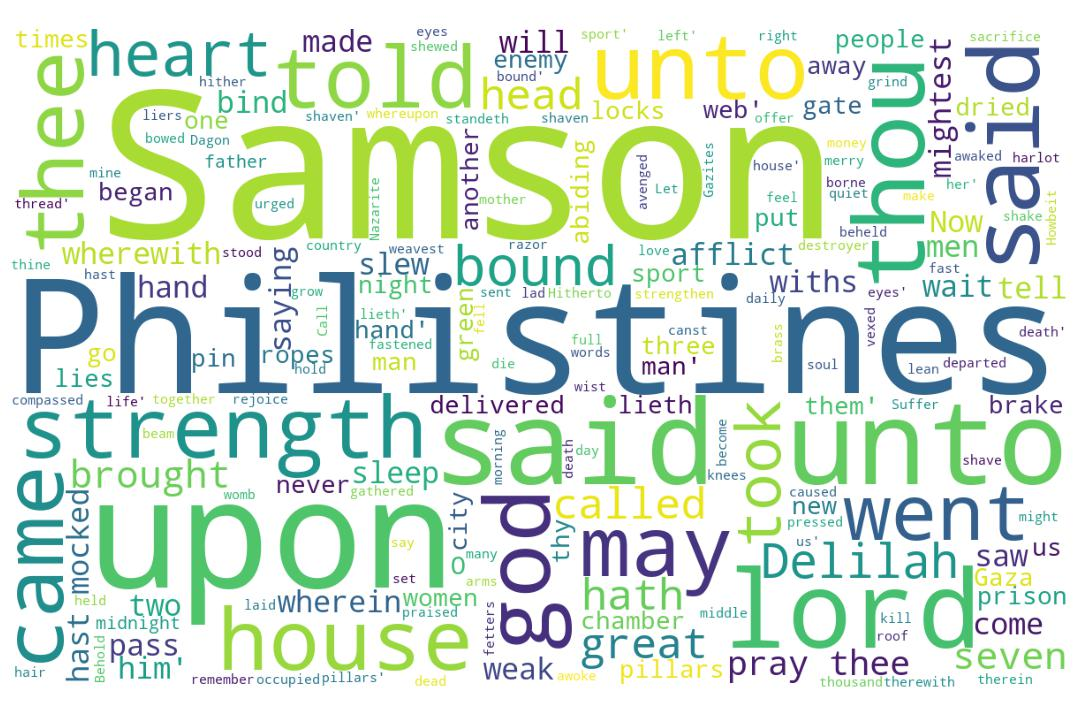
\includegraphics[width=\linewidth]{07OT-Judges/Judges16-WordCloud.jpg}
  \caption{Judges 16 Word Cloud}
  \label{fig:Judges 16 Word Cloud}
\end{figure}

\marginpar{\scriptsize \centering \fcolorbox{bone}{lime}{SAMSON'S END}\\ (Judges 16) \begin{compactenum}[I.][8]
    \item  His \textbf{Sweetheart} \index[scripture]{Judges!Jdg 16:04} (Jdg 16:4) 
    \item  His \textbf{Strength} \index[scripture]{Judges!Jdg 16:17} (Jdg 16:17) 
    \item  His \textbf{Seizure} \index[scripture]{Judges!Jdg 16:21} (Jdg 16:21) 
    \item  His Final \textbf{Scene} \index[scripture]{Judges!Jdg 16:3}(Jdg 16:31) 
    \item  His \textbf{Spirit} %\index[scripture]{Judges!Jdg 16:21} (Jdg 16:21) 
    \item  His \textbf{Scarcity} %\index[scripture]{Judges!Jdg 16:21} (Jdg 16:21) 
    \item  His \textbf{Shortcoming} %\index[scripture]{Judges!Jdg 16:21} (Jdg 16:21) 
\end{compactenum}}


\footnote{\textcolor[rgb]{0.00,0.25,0.00}{\hyperlink{JudgesTOC}{Return to end of Table of Contents.}}}\footnote{\href{https://audiobible.com/bible/judges_16.html}{\textcolor[cmyk]{0.99998,1,0,0}{Judges 16 Audio}}}\textcolor[cmyk]{0.99998,1,0,0}{Then went Samson to Gaza, and saw there an harlot, and went in unto her.}
[2] \textcolor[cmyk]{0.99998,1,0,0}{\emph{And} \emph{it} \emph{was} \emph{told} the Gazites, saying, Samson is come hither. And they compassed \emph{him} in, and laid wait for him all night in the gate of the city, and were quiet all the night, saying, In the morning, when it is day, we shall kill him.}
[3] \textcolor[cmyk]{0.99998,1,0,0}{And Samson lay till midnight, and arose at midnight, and took the doors of the gate of the city, and the two posts, and went away with them, bar and all, and put \emph{them} upon his shoulders, and carried them up to the top of an hill that \emph{is} before Hebron.}\\
\\
\P \textcolor[cmyk]{0.99998,1,0,0}{And it came to pass afterward, that he loved a woman in the valley of Sorek, whose name \emph{was} \fcolorbox{bone}{lime}{Delilah}.}
[5] \textcolor[cmyk]{0.99998,1,0,0}{And the lords of the \fcolorbox{bone}{bone}{Philistines} came up unto her, and said unto her, Entice him, and see wherein his great strength \emph{lieth}, and by what \emph{means} we may prevail against him, that we may bind him to afflict him: and we will give thee every one of us eleven hundred \emph{pieces} of silver.}\\
\\
\P \textcolor[cmyk]{0.99998,1,0,0}{And Delilah said to Samson, Tell me, I pray thee, wherein thy great strength \emph{lieth}, and wherewith thou mightest be bound to afflict thee.}
[7] \textcolor[cmyk]{0.99998,1,0,0}{And Samson said unto her, If they bind me with seven green withs that were never dried, then shall I be weak, and be as another man.}
[8] \textcolor[cmyk]{0.99998,1,0,0}{Then the lords of the \fcolorbox{bone}{bone}{Philistines} brought up to her seven green withs which had not been dried, and she bound him with them.}
[9] \textcolor[cmyk]{0.99998,1,0,0}{Now \emph{there} \emph{were} men lying in wait, abiding with her in the chamber. And she said unto him, The \fcolorbox{bone}{bone}{Philistines} \emph{be} upon thee, Samson. And he brake the withs, as a thread of tow is broken when it toucheth the fire. So his strength was not known.}
[10] \textcolor[cmyk]{0.99998,1,0,0}{And Delilah said unto Samson, Behold, thou hast mocked me, and told me lies: now tell me, I pray thee, wherewith thou mightest be bound.}
[11] \textcolor[cmyk]{0.99998,1,0,0}{And he said unto her, If they bind me fast with new ropes that never were occupied, then shall I be weak, and be as another man.}
[12] \textcolor[cmyk]{0.99998,1,0,0}{Delilah therefore took new ropes, and bound him therewith, and said unto him, The \fcolorbox{bone}{bone}{Philistines} \emph{be} upon thee, Samson. And \emph{there} \emph{were} liers in wait abiding in the chamber. And he brake them from off his arms like a thread.}
[13] \textcolor[cmyk]{0.99998,1,0,0}{And Delilah said unto Samson, Hitherto thou hast mocked me, and told me lies: tell me wherewith thou mightest be bound. And he said unto her, If thou weavest the seven locks of my head with the web.}
[14] \textcolor[cmyk]{0.99998,1,0,0}{And she fastened \emph{it} with the pin, and said unto him, The \fcolorbox{bone}{bone}{Philistines} \emph{be} upon thee, Samson. And he awaked out of his sleep, and went away with the pin of the beam, and with the web.}\\
\\
\P \textcolor[cmyk]{0.99998,1,0,0}{And she said unto him, How canst thou say, I love thee, when thine heart \emph{is} not with me? thou hast mocked me these three times, and hast not told me wherein thy great strength \emph{lieth}.}
[16] \textcolor[cmyk]{0.99998,1,0,0}{And it came to pass, when she pressed him daily with her words, and urged him, \emph{so} that his soul was vexed unto death;}
[17] \textcolor[cmyk]{0.99998,1,0,0}{That he told her all his heart, and said unto her, There hath not come a razor upon mine head; for I \emph{have} \emph{been} a Nazarite unto God from my mother's womb: if I be shaven, then my \fcolorbox{bone}{lime}{strength} will go from me, and I shall become weak, and be like any \emph{other} man.}
[18] \textcolor[cmyk]{0.99998,1,0,0}{And when Delilah saw that he had told her all his heart, she sent and called for the lords of the \fcolorbox{bone}{bone}{Philistines}, saying, Come up this once, for he hath shewed me all his heart. Then the lords of the \fcolorbox{bone}{bone}{Philistines} came up unto her, and brought money in their hand.}
[19] \textcolor[cmyk]{0.99998,1,0,0}{And she made him sleep upon her knees; and she called for a man, and she caused him to shave off the seven locks of his head; and she began to afflict him, and his strength went from him.}
[20] \textcolor[cmyk]{0.99998,1,0,0}{And she said, The \fcolorbox{bone}{bone}{Philistines} \emph{be} upon thee, Samson. And he awoke out of his sleep, and said, I will go out as at other times before, and shake myself. And he wist not that the LORD was departed from him.}\\
\\
\P \textcolor[cmyk]{0.99998,1,0,0}{But the \fcolorbox{bone}{bone}{Philistines} took him, and put out his eyes, and brought him down to Gaza, and \fcolorbox{bone}{lime}{bound} him with fetters of brass; and he did grind in the prison house.}
[22] \textcolor[cmyk]{0.99998,1,0,0}{Howbeit the hair of his head began to grow again after he was shaven.}
[23] \textcolor[cmyk]{0.99998,1,0,0}{Then the lords of the \fcolorbox{bone}{bone}{Philistines} gathered them together for to offer a great sacrifice unto Dagon their god, and to rejoice: for they said, Our god hath delivered Samson our enemy into our hand.}
[24] \textcolor[cmyk]{0.99998,1,0,0}{And when the people saw him, they praised their god: for they said, Our god hath delivered into our hands our enemy, and the destroyer of our country, which slew many of us.}
[25] \textcolor[cmyk]{0.99998,1,0,0}{And it came to pass, when their hearts were merry, that they said, Call for Samson, that he may make us sport. And they called for Samson out of the prison house; and he made them sport: and they set him between the pillars.}
[26] \textcolor[cmyk]{0.99998,1,0,0}{And Samson said unto the lad that held him by the hand, Suffer me that I may feel the pillars whereupon the house standeth, that I may lean upon them.}
[27] \textcolor[cmyk]{0.99998,1,0,0}{Now the house was full of men and women; and all the lords of the \fcolorbox{bone}{bone}{Philistines} \emph{were} there; and \emph{there} \emph{were} upon the roof about three thousand men and women, that beheld while Samson made sport.}
[28] \textcolor[cmyk]{0.99998,1,0,0}{And Samson called unto the LORD, and said, O Lord GOD, remember me, I pray thee, and strengthen me, I pray thee, only this once, O God, that I may be at once avenged of the \fcolorbox{bone}{bone}{Philistines} for my two eyes.}
[29] \textcolor[cmyk]{0.99998,1,0,0}{And Samson took hold of the two middle pillars upon which the house stood, and on which it was borne up, of the one with his right hand, and of the other with his left.}
[30] \textcolor[cmyk]{0.99998,1,0,0}{And Samson said, Let me die with the \fcolorbox{bone}{bone}{Philistines}. And he bowed himself with \emph{all} \emph{his} might; and the house fell upon the lords, and upon all the people that \emph{were} therein. So the dead which he slew at his death were more than \emph{they} which he slew in his life.}
[31] \textcolor[cmyk]{0.99998,1,0,0}{Then his brethren and all the house of his father came down, and took him, and brought \emph{him} up, and buried him between Zorah and Eshtaol in the \fcolorbox{bone}{lime}{buryingplace} of Manoah his father. And he judged Israel twenty years.}
\chapter{Judges 17}

\begin{figure}
  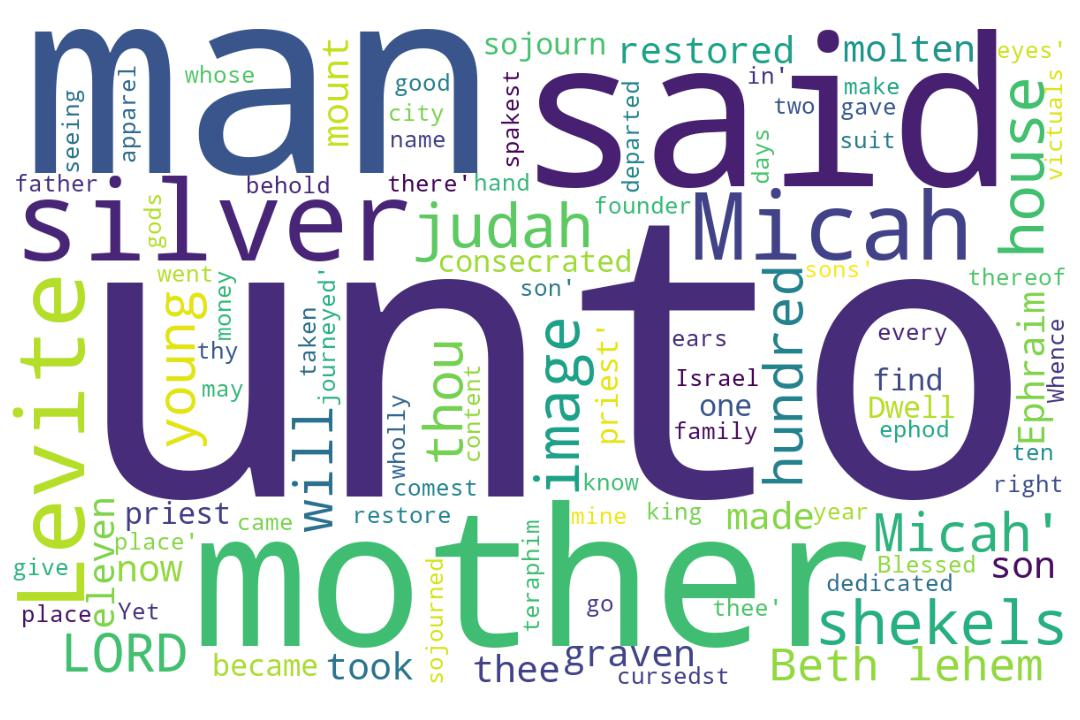
\includegraphics[width=\linewidth]{07OT-Judges/Judges17-WordCloud.jpg}
  \caption{Judges 17 Word Cloud}
  \label{fig:Judges 17 Word Cloud}
\end{figure}

\marginpar{\scriptsize \centering \fcolorbox{bone}{lime}{BUYING A PRIEST}\\ (Judges 17) \begin{compactenum}[I.][8]
    \item  The \textbf{Silver} \index[scripture]{Judges!Jdg 17:02} (Jdg 17:2) 
    \item  A \textbf{Statue} \index[scripture]{Judges!Jdg 17:04} (Jdg 17:4) 
    \item  A \textbf{Shrine} \index[scripture]{Judges!Jdg 17:05} (Jdg 17:5) 
    \item  The \textbf{Selection} \index[scripture]{Judges!Jdg 17:05} (Jdg 17:5) 
    \item  The \textbf{Sojourning} \index[scripture]{Judges!Jdg 17:07} (Jdg 17:7) 
    \item  The \textbf{Salary} \index[scripture]{Judges!Jdg 17:10} (Jdg 17:10) 
    \item  \textbf{Situational Reasoning} %\index[scripture]{Judges!Judges 17:05} (Jdg 17:5) 
\end{compactenum}}



\footnote{\textcolor[rgb]{0.00,0.25,0.00}{\hyperlink{TOC}{Return to end of Table of Contents.}}}\footnote{\href{https://audiobible.com/bible/judges_17.html}{\textcolor[cmyk]{0.99998,1,0,0}{Judges 17 Audio}}}\textcolor[cmyk]{0.99998,1,0,0}{And there was a man of mount Ephraim, whose name \emph{was} Micah.}
[2] \textcolor[cmyk]{0.99998,1,0,0}{And he said unto his mother, The eleven hundred \emph{shekels} of \fcolorbox{bone}{lime}{silver} that were taken from thee, about which thou cursedst, and spakest of also in mine ears, behold, the silver \emph{is} with me; I took it. And his mother said, Blessed \emph{be} \emph{thou} of the LORD, my son.}
[3] \textcolor[cmyk]{0.99998,1,0,0}{And when he had restored the eleven hundred \emph{shekels} of silver to his mother, his mother said, I had wholly dedicated the silver unto the LORD from my hand for my son, to make a graven image and a molten image: now therefore I will restore it unto thee.}
[4] \textcolor[cmyk]{0.99998,1,0,0}{Yet he restored the money unto his mother; and his mother took two hundred \emph{shekels} of silver, and gave them to the founder, who made thereof a graven image and a molten \fcolorbox{bone}{lime}{image}: and they were in the house of Micah.}
[5] \textcolor[cmyk]{0.99998,1,0,0}{And the man Micah had an \fcolorbox{bone}{lime}{house} of gods, and made an ephod, and teraphim, and consecrated one of his \fcolorbox{bone}{lime}{sons}, who became his priest.}
[6] \textcolor[cmyk]{0.99998,1,0,0}{In those days \emph{there} \emph{was} no king in Israel, \emph{but} every man did \emph{that} \emph{which} \emph{was} right in his own eyes.}\\
\\
\P\textcolor[cmyk]{0.99998,1,0,0}{And there was a young man out of Beth-lehem-judah of the family of Judah, who \emph{was} a Levite, and he \fcolorbox{bone}{lime}{sojourned} there.}
[8] \textcolor[cmyk]{0.99998,1,0,0}{And the man departed out of the city from Beth-lehem-judah to sojourn where he could find \emph{a} \emph{place}: and he came to mount Ephraim to the house of Micah, as he journeyed.}
[9] \textcolor[cmyk]{0.99998,1,0,0}{And Micah said unto him, Whence comest thou? And he said unto him, I \emph{am} a Levite of Beth-lehem-judah, and I go to sojourn where I may find \emph{a} \emph{place}.}
[10] \textcolor[cmyk]{0.99998,1,0,0}{And Micah said unto him, Dwell with me, and be unto me a father and a priest, and I will give thee ten \fcolorbox{bone}{lime}{\emph{shekels}} of silver by the year, and a suit of apparel, and thy victuals. So the Levite went in.}
[11] \textcolor[cmyk]{0.99998,1,0,0}{And the Levite was content to dwell with the man; and the young man was unto him as one of his sons.}
[12] \textcolor[cmyk]{0.99998,1,0,0}{And Micah consecrated the Levite; and the young man became his priest, and was in the house of Micah.}
[13] \textcolor[cmyk]{0.99998,1,0,0}{Then said Micah, Now know I that the LORD will do me good, \fcolorbox{bone}{lime}{\emph{seeing}} I have a Levite to \emph{my} priest.}
\chapter{Judges 18}

\begin{figure}
  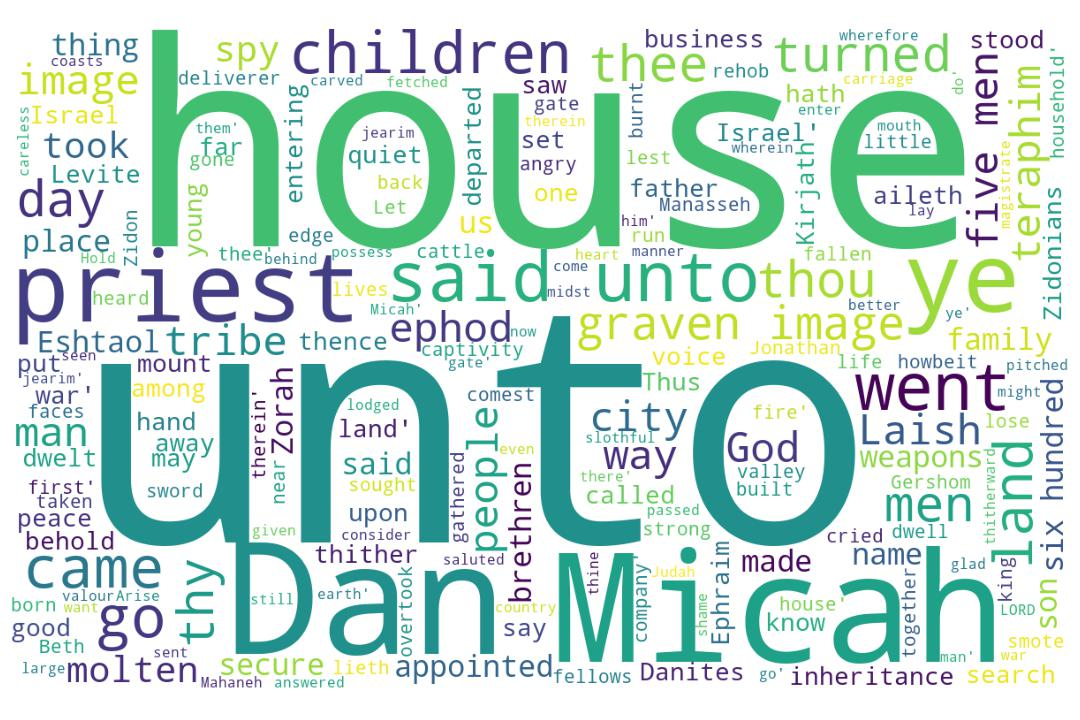
\includegraphics[width=\linewidth]{07OT-Judges/Judges18-WordCloud.jpg}
  \caption{Judges 18 Word Cloud}
  \label{fig:Judges 18 Word Cloud}
\end{figure}

\marginpar{\scriptsize \centering \fcolorbox{bone}{lime}{NEW HOME, NEW RELIGION}\\ (Judges 18) \begin{compactenum}[I.][8]
    \item The \textbf{Problem} \index[scripture]{Judges!Jdg 18:01}(Jdg 18:1)
    \item Looking for a  \textbf{Place} \index[scripture]{Judges!Jdg 18:01}(Jdg 18:1)
    \item The \textbf{Prayer} \index[scripture]{Judges!Jdg 18:05}(Jdg 18:5)
    \item A \textbf{Prognosis} \index[scripture]{Judges!Jdg 18:08}(Jdg 18:8)
    \item A \textbf{Plan} \index[scripture]{Judges!Jdg 18:09}(Jdg 18:9)
    \item A \textbf{Promotion} \index[scripture]{Judges!Jdg 18:20}(Jdg 18:20)
    \item A Religion \textbf{Put} in Place \index[scripture]{Judges!Jdg 18:30}(Jdg 18:30)
\end{compactenum}}




\footnote{\textcolor[rgb]{0.00,0.25,0.00}{\hyperlink{TOC}{Return to end of Table of Contents.}}}\footnote{\href{https://audiobible.com/bible/judges_18.html}{\textcolor[cmyk]{0.99998,1,0,0}{Judges 18 Audio}}}\textcolor[cmyk]{0.99998,1,0,0}{In those days \emph{there} \emph{was} \fcolorbox{bone}{lime}{no king in Israel}: and in those days the tribe of the Danites \fcolorbox{bone}{lime}{sought them an inheritance} to dwell in; for unto that day \emph{all} \emph{their} inheritance had not fallen unto them among the tribes of Israel.}
[2] \textcolor[cmyk]{0.99998,1,0,0}{And the children of Dan sent of their family five men from their coasts, men of valour, from Zorah, and from Eshtaol, to spy out the land, and to search it; and they \fcolorbox{bone}{bone}{said} unto them, Go, search the land: who when they came to mount Ephraim, to the house of Micah, they lodged there.}
[3] \textcolor[cmyk]{0.99998,1,0,0}{When they \emph{were} by the house of Micah, they knew the voice of the young man the Levite: and they turned in thither, and \fcolorbox{bone}{bone}{said} unto him, Who brought thee hither? and what makest thou in this \emph{place}? and what hast thou here?}
[4] \textcolor[cmyk]{0.99998,1,0,0}{And he \fcolorbox{bone}{bone}{said} unto them, Thus and thus dealeth Micah with me, and hath hired me, and I am his priest.}
[5] \textcolor[cmyk]{0.99998,1,0,0}{\fcolorbox{bone}{bone}{And they} \fcolorbox{bone}{bone}{said} unto him, Ask counsel, we \fcolorbox{bone}{lime}{pray} thee, of God, that we may know whether our way which we go shall be prosperous.}
[6] \textcolor[cmyk]{0.99998,1,0,0}{And the priest \fcolorbox{bone}{bone}{said} unto them, Go in peace: before the LORD \emph{is} your way wherein ye go.}\\
\\
\P \textcolor[cmyk]{0.99998,1,0,0}{Then the five men departed, and came to Laish, and saw the people that \emph{were} therein, how they dwelt careless, after the manner of the Zidonians, quiet and secure; and \emph{there} \emph{was} no magistrate in the land, that might put \emph{them} to shame in \emph{any} thing; and they \emph{were} far from the Zidonians, and had no business with \emph{any} man.}
[8] \textcolor[cmyk]{0.99998,1,0,0}{\fcolorbox{bone}{bone}{And they} came unto their brethren to Zorah and Eshtaol: and their brethren \fcolorbox{bone}{bone}{said} unto them, \fcolorbox{bone}{lime}{What \emph{say} ye}?}
[9] \textcolor[cmyk]{0.99998,1,0,0}{\fcolorbox{bone}{bone}{And they} \fcolorbox{bone}{bone}{said}, Arise, that we may go up against them: for we have seen the land, and, behold, it \emph{is} very good: and \emph{are} ye still? be not slothful to go, \emph{and} to \fcolorbox{bone}{lime}{enter to possess} the land.}
[10] \textcolor[cmyk]{0.99998,1,0,0}{When ye go, ye shall come unto a people secure, and to a large land: for God hath given it into your hands; a place where \emph{there} \emph{is} no want of any thing that \emph{is} in the earth.}\\
\\
\P \textcolor[cmyk]{0.99998,1,0,0}{And there went from thence of the family of the Danites, out of Zorah and out of Eshtaol, six hundred men appointed with weapons of war.}
[12] \textcolor[cmyk]{0.99998,1,0,0}{\fcolorbox{bone}{bone}{And they} went up, and pitched in Kirjath-jearim, in Judah: wherefore they called that place Mahaneh-dan unto this day: behold, \emph{it} \emph{is} behind Kirjath-jearim.}
[13] \textcolor[cmyk]{0.99998,1,0,0}{\fcolorbox{bone}{bone}{And they} passed thence unto mount Ephraim, and came unto the house of Micah.}\\
\\
\P \textcolor[cmyk]{0.99998,1,0,0}{Then answered the five men that went to spy out the country of Laish, and \fcolorbox{bone}{bone}{said} unto their brethren, Do ye know that there is in these houses an ephod, and teraphim, and a graven image, and a molten image? now therefore consider what ye have to do.}
[15] \textcolor[cmyk]{0.99998,1,0,0}{\fcolorbox{bone}{bone}{And they} turned thitherward, and came to the house of the young man the Levite, \emph{even} unto the house of Micah, and saluted him.}
[16] \textcolor[cmyk]{0.99998,1,0,0}{And the six hundred men appointed with their weapons of war, which \emph{were} of the children of Dan, stood by the entering of the gate.}
[17] \textcolor[cmyk]{0.99998,1,0,0}{And the five men that went to spy out the land went up, \emph{and} came in thither, \emph{and} took the graven image, and the ephod, and the teraphim, and the molten image: and the priest stood in the entering of the gate with the six hundred men \emph{that} \emph{were} appointed with weapons of war.}
[18] \textcolor[cmyk]{0.99998,1,0,0}{And these went into Micah's house, and fetched the carved image, the ephod, and the teraphim, and the molten image. Then \fcolorbox{bone}{bone}{said} the priest unto them, What do ye?}
[19] \textcolor[cmyk]{0.99998,1,0,0}{\fcolorbox{bone}{bone}{And they} \fcolorbox{bone}{bone}{said} unto him, Hold thy peace, lay thine hand upon thy mouth, and go with us, and be to us a father and a priest: \emph{is} \emph{it} better for thee to be a priest unto the house of one man, or that thou be a priest unto a tribe and a family in Israel?}
[20] \textcolor[cmyk]{0.99998,1,0,0}{And the priest's heart was glad, and he took the ephod, and the teraphim, and the graven image, and \fcolorbox{bone}{lime}{went} in the midst of the people.}
[21] \textcolor[cmyk]{0.99998,1,0,0}{So they turned and departed, and put the little ones and the cattle and the carriage before them.}\\
\\
\P \textcolor[cmyk]{0.99998,1,0,0}{\emph{And} when they were a good way from the house of Micah, the men that \emph{were} in the houses near to Micah's house were gathered together, and overtook the children of Dan.}
[23] \textcolor[cmyk]{0.99998,1,0,0}{\fcolorbox{bone}{bone}{And they} cried unto the children of Dan. \fcolorbox{bone}{bone}{And they} turned their faces, and \fcolorbox{bone}{bone}{said} unto Micah, What aileth thee, that thou comest with such a company?}
[24] \textcolor[cmyk]{0.99998,1,0,0}{And he \fcolorbox{bone}{bone}{said}, Ye have taken away my gods which I made, and the priest, and ye are gone away: and what have I more? and what \emph{is} this \emph{that} ye say unto me, What aileth thee?}
[25] \textcolor[cmyk]{0.99998,1,0,0}{And the children of Dan \fcolorbox{bone}{bone}{said} unto him, Let not thy voice be heard among us, lest angry fellows run upon thee, and thou lose thy life, with the lives of thy household.}
[26] \textcolor[cmyk]{0.99998,1,0,0}{And the children of Dan went their way: and when Micah saw that they \emph{were} too strong for him, he turned and went back unto his house.}
[27] \textcolor[cmyk]{0.99998,1,0,0}{\fcolorbox{bone}{bone}{And they} took \emph{the} \emph{things} which Micah had made, and the priest which he had, and came unto Laish, unto a people \emph{that} \emph{were} at quiet and secure: and they smote them with the edge of the sword, and burnt the city with fire.}
[28] \textcolor[cmyk]{0.99998,1,0,0}{And \emph{there} \emph{was} no deliverer, because it \emph{was} far from Zidon, and they had no business with \emph{any} man; and it was in the valley that \emph{lieth} by Beth-rehob. \fcolorbox{bone}{bone}{And they} built a city, and dwelt therein.}
[29] \textcolor[cmyk]{0.99998,1,0,0}{\fcolorbox{bone}{bone}{And they} called the name of the city Dan, after the name of Dan their father, who was born unto Israel: howbeit the name of the city \emph{was} Laish at the first.}\\
\\
\P \textcolor[cmyk]{0.99998,1,0,0}{And the children of Dan set up the graven image: and Jonathan, the son of Gershom, the son of Manasseh, he and his sons were priests to the tribe of Dan until the day of the captivity of the land.}
[31] \textcolor[cmyk]{0.99998,1,0,0}{\fcolorbox{bone}{bone}{And they} set them up Micah's graven image, which he made, all the time that the house of God was in Shiloh.}

\chapter{Psalm 78}

\begin{figure}
  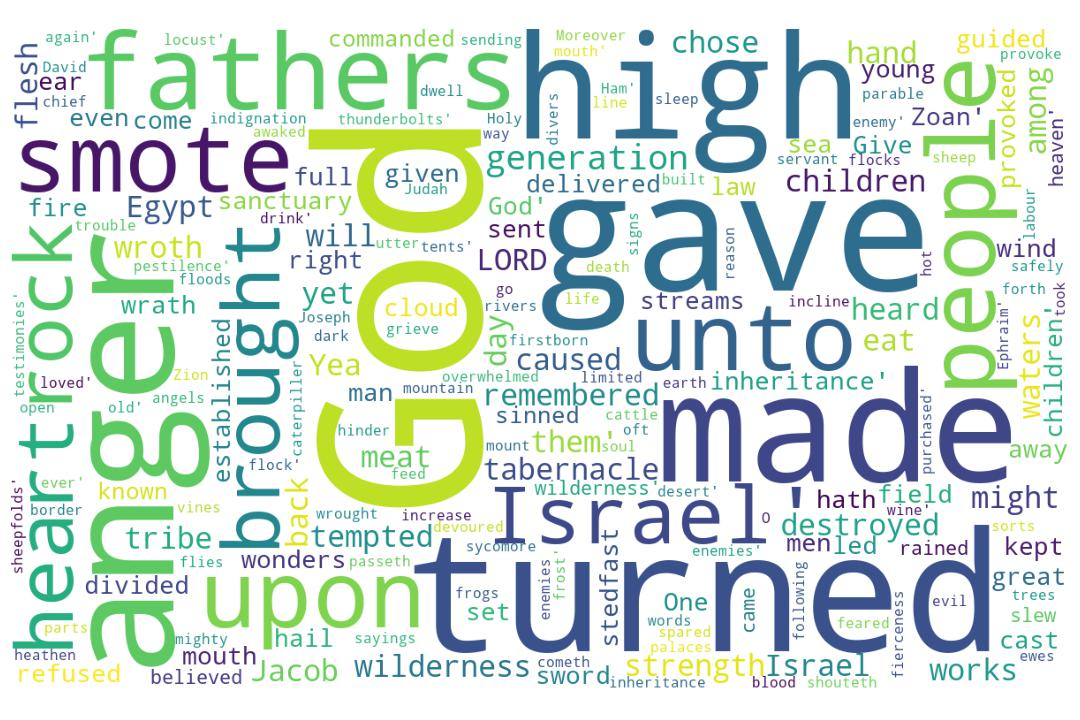
\includegraphics[width=\linewidth]{19OT-Psalms/Psalm78-WordCloud.jpg}
  \caption{Psalm 78 Word Cloud}
  \label{fig:Psalm 78 word Cloud}
\end{figure}

\marginpar{\scriptsize \centering \fcolorbox{bone}{lime}{\textbf{GOD AND HIS PEOPLE}}\\ (Psalm 77) \begin{compactenum}[I.][8]
    \item The  \textbf{Teaching}  \index[scripture]{Psalms!Psa 078:04}(Psa 78:4)
    \item The  \textbf{Testimony}  \index[scripture]{Psalms!Psa 078:05}(Psa 78:5)
    \item The  \textbf{Tempting}  \index[scripture]{Psalms!Psa 078:18}\index[scripture]{Psalms!Psa 078:56} (Psa 78:18, 56)
    \item The  \textbf{Turning}  \index[scripture]{Psalms!Psa 078:41}(Psa 78:41)
    \item The  \textbf{Transgressions}  %\index[scripture]{Psalms!Psa 078:05}(Psalm 78:5)
    \item The  \textbf{Tribe}  \index[scripture]{Psalms!Psa 078:68}(Psa 78:68)
    \item The  \textbf{Tenderness}  \index[scripture]{Psalms!Psa 078:72}(Psa 78:72)
\end{compactenum}}
    




% \textcolor[cmyk]{0.99998,1,0,0}{
\footnote{\textcolor[rgb]{0.00,0.25,0.00}{\hyperlink{TOC}{Return to end of Table of Contents.}}}\footnote{\href{https://audiobible.com/bible/psalms_78.html}{\textcolor[cmyk]{0.99998,1,0,0}{Psalm 78 Audio}}}\textcolor[cmyk]{0.99998,1,0,0}{Maschil of Asaph}\\
\\
\textcolor[cmyk]{0.99998,1,0,0}{Give ear, O my people, \emph{to} my law: incline your ears to the words of my mouth.}
[2] \textcolor[cmyk]{0.99998,1,0,0}{I will open my mouth in a parable: I will utter dark sayings of old:}
[3] \textcolor[cmyk]{0.99998,1,0,0}{Which we have heard and known, and our fathers have told us.}
[4] \textcolor[cmyk]{0.99998,1,0,0}{We will not hide \emph{them} from their children, shewing to the \fcolorbox{bone}{lime}{generation to come} the praises of the LORD, and his strength, and his wonderful works that he hath done.}
[5] \textcolor[cmyk]{0.99998,1,0,0}{For he established a \fcolorbox{bone}{lime}{testimony} in Jacob, and appointed a law in Israel, which he commanded our fathers, that they should make them known to their children:}
[6] \textcolor[cmyk]{0.99998,1,0,0}{That the generation to come might know \emph{them,} \emph{even} the children \emph{which} should be born; \emph{who} should arise and declare \emph{them} to their children:}
[7] \textcolor[cmyk]{0.99998,1,0,0}{That they might set their hope in God, and not forget the works of God, but keep his commandments:}
[8] \textcolor[cmyk]{0.99998,1,0,0}{And might not be as their fathers, a stubborn and rebellious generation; a generation \emph{that} set not their heart aright, and whose spirit was not stedfast with God.}
[9] \textcolor[cmyk]{0.99998,1,0,0}{The children of Ephraim, \emph{being} armed, \emph{and} carrying bows, turned back in the day of battle.}
[10] \textcolor[cmyk]{0.99998,1,0,0}{They kept not the covenant of God, and refused to walk in his law;}
[11] \textcolor[cmyk]{0.99998,1,0,0}{And forgat his works, and his wonders that he had shewed them.}
[12] \textcolor[cmyk]{0.99998,1,0,0}{Marvellous things did he in the sight of their fathers, in the land of Egypt, \emph{in} the field of Zoan.}
[13] \textcolor[cmyk]{0.99998,1,0,0}{He divided the sea, and caused them to pass through; and he made the waters to stand as an heap.}
[14] \textcolor[cmyk]{0.99998,1,0,0}{In the daytime also he led them with a cloud, and all the night with a light of fire.}
[15] \textcolor[cmyk]{0.99998,1,0,0}{He clave the rocks in the wilderness, and gave \emph{them} drink as \emph{out} \emph{of} the great depths.}
[16] \textcolor[cmyk]{0.99998,1,0,0}{He brought streams also out of the rock, and caused waters to run down like rivers.}
[17] \textcolor[cmyk]{0.99998,1,0,0}{And they sinned yet more against him by provoking the most High in the wilderness.}
[18] \textcolor[cmyk]{0.99998,1,0,0}{And they \fcolorbox{bone}{lime}{tempted} God in their heart by asking meat for their lust.}
[19] \textcolor[cmyk]{0.99998,1,0,0}{Yea, they spake against God; they said, Can God furnish a table in the wilderness?}
[20] \textcolor[cmyk]{0.99998,1,0,0}{Behold, he smote the rock, that the waters gushed out, and the streams overflowed; can he give bread also? can he provide flesh for his people?}
[21] \textcolor[cmyk]{0.99998,1,0,0}{Therefore the LORD heard \emph{this}, and was wroth: so a fire was kindled against Jacob, and anger also came up against Israel;}
[22] \textcolor[cmyk]{0.99998,1,0,0}{Because they believed not in God, and trusted not in his salvation:}
[23] \textcolor[cmyk]{0.99998,1,0,0}{Though he had commanded the clouds from above, and opened the doors of heaven,}
[24] \textcolor[cmyk]{0.99998,1,0,0}{And had rained down manna upon them to eat, and had given them of the corn of heaven.}
[25] \textcolor[cmyk]{0.99998,1,0,0}{Man did eat angels' food: he sent them meat to the full.}
[26] \textcolor[cmyk]{0.99998,1,0,0}{He caused an east wind to blow in the heaven: and by his power he brought in the south wind.}
[27] \textcolor[cmyk]{0.99998,1,0,0}{He rained flesh also upon them as dust, and feathered fowls like as the sand of the sea:}
[28] \textcolor[cmyk]{0.99998,1,0,0}{And he let \emph{it} fall in the midst of their camp, round about their habitations.}
[29] \textcolor[cmyk]{0.99998,1,0,0}{So they did eat, and were well filled: for he gave them their own desire;}
[30] \textcolor[cmyk]{0.99998,1,0,0}{They were not estranged from their lust. But while their meat \emph{was} yet in their mouths,}
[31] \textcolor[cmyk]{0.99998,1,0,0}{The wrath of God came upon them, and slew the fattest of them, and smote down the chosen \emph{men} of Israel.}
[32] \textcolor[cmyk]{0.99998,1,0,0}{For all this they sinned still, and believed not for his wondrous works.}
[33] \textcolor[cmyk]{0.99998,1,0,0}{Therefore their days did he consume in vanity, and their years in trouble.}
[34] \textcolor[cmyk]{0.99998,1,0,0}{When he slew them, then they sought him: and they returned and enquired early after God.}
[35] \textcolor[cmyk]{0.99998,1,0,0}{And they remembered that God \emph{was} their rock, and the high God their redeemer.}
[36] \textcolor[cmyk]{0.99998,1,0,0}{Nevertheless they did flatter him with their mouth, and they lied unto him with their tongues.}
[37] \textcolor[cmyk]{0.99998,1,0,0}{For their heart was not right with him, neither were they stedfast in his covenant.}
[38] \textcolor[cmyk]{0.99998,1,0,0}{But he, \emph{being} full of compassion, forgave \emph{their} iniquity, and destroyed \emph{them} not: yea, many a time turned he his anger away, and did not stir up all his wrath.}
[39] \textcolor[cmyk]{0.99998,1,0,0}{For he remembered that they \emph{were} \emph{but} flesh; a wind that passeth away, and cometh not again.}
[40] \textcolor[cmyk]{0.99998,1,0,0}{How oft did they provoke him in the wilderness, \emph{and} grieve him in the desert!}
[41] \textcolor[cmyk]{0.99998,1,0,0}{Yea, they \fcolorbox{bone}{lime}{turned} back and tempted God, and limited the Holy One of Israel.}
[42] \textcolor[cmyk]{0.99998,1,0,0}{They remembered not his hand, \emph{nor} the day when he delivered them from the enemy.}
[43] \textcolor[cmyk]{0.99998,1,0,0}{How he had wrought his signs in Egypt, and his wonders in the field of Zoan:}
[44] \textcolor[cmyk]{0.99998,1,0,0}{And had turned their rivers into blood; and their floods, that they could not drink.}
[45] \textcolor[cmyk]{0.99998,1,0,0}{He sent divers sorts of flies among them, which devoured them; and frogs, which destroyed them.}
[46] \textcolor[cmyk]{0.99998,1,0,0}{He gave also their increase unto the caterpiller, and their labour unto the locust.}
[47] \textcolor[cmyk]{0.99998,1,0,0}{He destroyed their vines with hail, and their sycomore trees with frost.}
[48] \textcolor[cmyk]{0.99998,1,0,0}{He gave up their cattle also to the hail, and their flocks to hot thunderbolts.}
[49] \textcolor[cmyk]{0.99998,1,0,0}{He cast upon them the fierceness of his anger, wrath, and indignation, and trouble, by sending evil angels \emph{among} \emph{them}.}
[50] \textcolor[cmyk]{0.99998,1,0,0}{He made a way to his anger; he spared not their soul from death, but gave their life over to the pestilence;}
[51] \textcolor[cmyk]{0.99998,1,0,0}{And smote all the firstborn in Egypt; the chief of \emph{their} strength in the tabernacles of Ham:}
[52] \textcolor[cmyk]{0.99998,1,0,0}{But made his own people to go forth like sheep, and guided them in the wilderness like a flock.}
[53] \textcolor[cmyk]{0.99998,1,0,0}{And he led them on safely, so that they feared not: but the sea overwhelmed their enemies.}
[54] \textcolor[cmyk]{0.99998,1,0,0}{And he brought them to the border of his sanctuary, \emph{even} \emph{to} this mountain, \emph{which} his right hand had purchased.}
[55] \textcolor[cmyk]{0.99998,1,0,0}{He cast out the heathen also before them, and divided them an inheritance by line, and made the tribes of Israel to dwell in their tents.}
[56] \textcolor[cmyk]{0.99998,1,0,0}{Yet they \fcolorbox{bone}{lime}{tempted} and provoked the most high God, and kept not his testimonies:}
[57] \textcolor[cmyk]{0.99998,1,0,0}{But turned back, and dealt unfaithfully like their fathers: they were turned aside like a deceitful bow.}
[58] \textcolor[cmyk]{0.99998,1,0,0}{For they provoked him to anger with their high places, and moved him to jealousy with their graven images.}
[59] \textcolor[cmyk]{0.99998,1,0,0}{When God heard \emph{this}, he was wroth, and greatly abhorred Israel:}
[60] \textcolor[cmyk]{0.99998,1,0,0}{So that he forsook the tabernacle of Shiloh, the tent \emph{which} he placed among men;}
[61] \textcolor[cmyk]{0.99998,1,0,0}{And delivered his strength into captivity, and his glory into the enemy's hand.}
[62] \textcolor[cmyk]{0.99998,1,0,0}{He gave his people over also unto the sword; and was wroth with his inheritance.}
[63] \textcolor[cmyk]{0.99998,1,0,0}{The fire consumed their young men; and their maidens were not given to marriage.}
[64] \textcolor[cmyk]{0.99998,1,0,0}{Their priests fell by the sword; and their widows made no lamentation.}
[65] \textcolor[cmyk]{0.99998,1,0,0}{Then the Lord awaked as one out of sleep, \emph{and} like a mighty man that shouteth by reason of wine.}
[66] \textcolor[cmyk]{0.99998,1,0,0}{And he smote his enemies in the hinder parts: he put them to a perpetual reproach.}
[67] \textcolor[cmyk]{0.99998,1,0,0}{Moreover he refused the tabernacle of Joseph, and chose not the tribe of Ephraim:}
[68] \textcolor[cmyk]{0.99998,1,0,0}{But chose the \fcolorbox{bone}{lime}{tribe} of Judah, the mount Zion which he loved.}
[69] \textcolor[cmyk]{0.99998,1,0,0}{And he built his sanctuary like high \emph{palaces}, like the earth which he hath established for ever.}
[70] \textcolor[cmyk]{0.99998,1,0,0}{He chose David also his servant, and took him from the sheepfolds:}
[71] \textcolor[cmyk]{0.99998,1,0,0}{From following the ewes great with young he brought him to feed Jacob his people, and Israel his inheritance.}
[72] \textcolor[cmyk]{0.99998,1,0,0}{So he fed them according to the integrity of his heart; and guided them by the \fcolorbox{bone}{lime}{skilfulness} of his hands.}

\chapter{Proverb 19}
\begin{figure}
  \includegraphics[width=\linewidth]{20OT-Proverbs/Proverb19-Wordcloud.jpg}
  \caption{Proverb 19 Word Cloud}
  \label{fig:Proverb 19 word Cloud}
\end{figure}

\marginpar{\scriptsize \centering \fcolorbox{bone}{lime}{\textbf{THE BASICS OF LIFE}}\\ (Proverbs 19:1-29) \begin{compactenum}[I.][8]
    \item \textbf{Wealth} \index[scripture]{Proverbs!Pro 19:01} \index[scripture]{Proverbs!Pro 19:17}(Pro 19:1, 17)
    \item \textbf{Words} \index[scripture]{Proverbs!Pro 19:01}\index[scripture]{Proverbs!Pro 19:07} \index[scripture]{Proverbs!Pro 19:29}(Pro 19:1, 7, 29)
    \item \textbf{Witness}  \index[scripture]{Proverbs!Pro 19:05} \index[scripture]{Proverbs!Pro 19:28}(Pro 19:5, 28)
    \item \textbf{Wisdom} \index[scripture]{Proverbs!Pro 19:02}\index[scripture]{Proverbs!Pro 19:08} \index[scripture]{Proverbs!Pro 19:27} (Pro 19:2, 8, 27)
    \item \textbf{Women} \index[scripture]{Proverbs!Pro 19:14}(Pro 19:14)
    \item \textbf{Ways} \index[scripture]{Proverbs!Pro 19:16}(Pro 19:16)
    \item \textbf{Work} \index[scripture]{Proverbs!Pro 19:24}(Pro 19:24)
\end{compactenum}}

\marginpar{\scriptsize \centering \fcolorbox{bone}{yellow}{\textbf{SMALL, BUT THEY MATTER}}\\ (Proverbs 19:1-29) \begin{compactenum}[I.][8]
    \item A Man's \textbf{Discernment} \index[scripture]{Proverbs!Pro 19:08}(Pro 19:8)
    \item A Man's \textbf{Delight} \index[scripture]{Proverbs!Pro 19:10}(Pro 19:10)
    \item A Man's \textbf{Discretion} \index[scripture]{Proverbs!Pro 19:11}(Pro 19:11)
    \item A Man's \textbf{Direction} \index[scripture]{Proverbs!Pro 19:16} \index[scripture]{Proverbs!Pro 19:27}(Pro 19:16, 19:27)
    \item A Man's \textbf{Devices} \index[scripture]{Proverbs!Prov 19:21}(Pro 19:21)
    \item A Man's \textbf{Desire} \index[scripture]{Proverbs!Prov 19:22}(Pro 19:22)
    \item A Man's \textbf{Discipline} \index[scripture]{Proverbs!Pro 19:29}(Pro 19:29)
\end{compactenum}}


\marginpar{\scriptsize \centering \fcolorbox{black}{black}{\textbf{\textcolor[cmyk]{0,0,0,0}{NEGATIVE THINGS}}}\\ (Proverbs 19:1-29) \begin{compactenum}[I.][8]
    \item \textbf{Foolish Lips} \index[scripture]{Proverbs!Pro 19:01}(Pro 19:1)
    \item \textbf{Feet that lead Astray} \index[scripture]{Proverbs!Pro 19:02}(Pro 19:2)
    \item A \textbf{Fretting Heart} \index[scripture]{Proverbs!Pro 19:03}(Pro 19:3)
    \item \textbf{Friends only in the Good Times} \index[scripture]{Proverbs!Pro 19:04}\index[scripture]{Proverbs!Pro 19:06}\index[scripture]{Proverbs!Pro 19:07}(Pro 19:4, 6, 7)
    \item \textbf{False Witnesses} \index[scripture]{Proverbs!Pro 19:05}(Pro 19:5)
    \item \textbf{Undeferred Anger} \index[scripture]{Proverbs!Pro 19:11}(Pro 19:11)
    \item \textbf{Favor Not Found} \index[scripture]{Proverbs!Pro 19:12}(Pro 19:12)
\end{compactenum}}

\footnote{\textcolor[cmyk]{0.99998,1,0,0}{\hyperlink{TOC}{Return to end of Table of Contents.}}}\footnote{\href{https://audiobible.com/bible/proverbs_19.html}{\textcolor[cmyk]{0.99998,1,0,0}{Proverbs Audio}}}\textcolor[cmyk]{0.99998,1,0,0}{Better \emph{is} the \fcolorbox{bone}{lime}{poor} that walketh in his integrity, than \emph{he} \emph{that} \emph{is} perverse \fcolorbox{bone}{lime}{in his lips}, and is a fool.}\footnote{\textbf{Proverbs 28:6} - Better is the poor that walketh in his uprightness, than he that is perverse in his ways, though he be rich.} 
[2] \textcolor[cmyk]{0.99998,1,0,0}{Also, \emph{that} the soul \emph{be} without \fcolorbox{bone}{lime}{knowledge}, \emph{it} \emph{is} not good; and he that hasteth with \emph{his} feet sinneth.}\footnote{\textbf{Proverbs 28:22} - He that hasteth to be rich hath an evil eye, and considereth not that poverty shall come upon him.} 
[3] \textcolor[cmyk]{0.99998,1,0,0}{The foolishness of man perverteth his way: and his heart fretteth against the LORD.}\footnote{\textbf{Provers 10:9} - He that walketh uprightly walketh surely: but he that perverteth his ways shall be known.} 
[4] \textcolor[cmyk]{0.99998,1,0,0}{Wealth maketh many friends; but the poor is separated from his neighbour.}
[5] \textcolor[cmyk]{0.99998,1,0,0}{A false \fcolorbox{bone}{lime}{witness} shall not be unpunished, and \emph{he} \emph{that} speaketh lies shall not escape.}
[6] \textcolor[cmyk]{0.99998,1,0,0}{Many will intreat the favour of the prince: and every man \emph{is} a friend to him that giveth gifts.}
[7] \textcolor[cmyk]{0.99998,1,0,0}{All the brethren of the poor do hate him: how much more do his friends go far from him? he pursueth \emph{them} \emph{with} \fcolorbox{bone}{lime}{words}, \emph{yet} they \emph{are} wanting \emph{to} \emph{him}.}
[8] \textcolor[cmyk]{0.99998,1,0,0}{He that getteth \fcolorbox{bone}{lime}{wisdom} loveth his own soul: he that keepeth \fcolorbox{bone}{MYGOLD}{understanding} shall find good.}
[9] \textcolor[cmyk]{0.99998,1,0,0}{A false witness shall not be unpunished, and \emph{he} \emph{that} speaketh lies shall perish.}
[10] \textcolor[cmyk]{0.99998,1,0,0}{\fcolorbox{bone}{yellow}{Delight} is not seemly for a fool; much less for a servant to have rule over princes.}
[11] \textcolor[cmyk]{0.99998,1,0,0}{The \fcolorbox{bone}{yellow}{discretion} of a man deferreth his anger; and \emph{it} \emph{is} his glory to pass over a \fcolorbox{bone}{MYGOLD}{transgression}.}
[12] \textcolor[cmyk]{0.99998,1,0,0}{The king's wrath \emph{is} as the roaring of a lion; but his favour \emph{is} as dew upon the grass.}
[13] \textcolor[cmyk]{0.99998,1,0,0}{A foolish son \emph{is} the calamity of his father: and the contentions of a wife \emph{are} a continual dropping.}
[14] \textcolor[cmyk]{0.99998,1,0,0}{House and riches \emph{are} the inheritance of fathers: and a \fcolorbox{bone}{lime}{prudent wife} \emph{is} from the LORD.}
[15] \textcolor[cmyk]{0.99998,1,0,0}{Slothfulness casteth into a deep sleep; and an idle soul shall suffer hunger.}
[16] \textcolor[cmyk]{0.99998,1,0,0}{He that keepeth the \fcolorbox{bone}{yellow}{commandment} keepeth his own soul; \emph{but} he that despiseth his \fcolorbox{bone}{lime}{ways} shall die.}
[17] \textcolor[cmyk]{0.99998,1,0,0}{He that hath pity upon the \fcolorbox{bone}{lime}{poor} lendeth unto the LORD; and that which he hath given will he pay him again.}
[18] \textcolor[cmyk]{0.99998,1,0,0}{Chasten thy son while there is hope, and let not thy soul spare for his crying.}
[19] \textcolor[cmyk]{0.99998,1,0,0}{A man of great wrath shall suffer punishment: for if thou deliver \emph{him}, yet thou must do it again.}
[20] \textcolor[cmyk]{0.99998,1,0,0}{Hear counsel, and receive instruction, that thou mayest be wise in thy latter end.}
[21] \textcolor[cmyk]{0.99998,1,0,0}{\emph{There} \emph{are} many \fcolorbox{bone}{yellow}{devices} in a man's heart; nevertheless the counsel of the LORD, that shall stand.}
[22] \textcolor[cmyk]{0.99998,1,0,0}{The \fcolorbox{bone}{yellow}{desire} of a man \emph{is} his kindness: and a poor man \emph{is} better than a liar.}
[23] \textcolor[cmyk]{0.99998,1,0,0}{The fear of the LORD \emph{tendeth} to life: and \emph{he} \emph{that} \emph{hath} \emph{it} shall abide satisfied; he shall not be visited with evil.}
[24] \textcolor[cmyk]{0.99998,1,0,0}{A \fcolorbox{bone}{lime}{slothful} \emph{man} hideth his hand in \emph{his} bosom, and will not so much as bring it to his mouth again.}
[25] \textcolor[cmyk]{0.99998,1,0,0}{Smite a scorner, and the simple will beware: and reprove one that hath \fcolorbox{bone}{MYGOLD}{understanding}, \emph{and} he will understand knowledge.}
[26] \textcolor[cmyk]{0.99998,1,0,0}{He that wasteth \emph{his} father, \emph{and} chaseth away \emph{his} mother, \emph{is} a son that causeth shame, and bringeth reproach.}
[27] \textcolor[cmyk]{0.99998,1,0,0}{Cease, my son, to hear the instruction \emph{that} \emph{causeth} to err from the \fcolorbox{bone}{lime}{words of knowledge}.}
[28] \textcolor[cmyk]{0.99998,1,0,0}{An ungodly \fcolorbox{bone}{lime}{witness} scorneth judgment: and the mouth of the wicked devoureth iniquity.}
[29] \textcolor[cmyk]{0.99998,1,0,0}{\fcolorbox{bone}{yellow}{Judgments} are prepared for \fcolorbox{bone}{lime}{scorners}, and stripes for the back of fools.}




\end{document}

